\section{Retningsregulerende kreds}
\begin{figure}[H]	
	\centering
    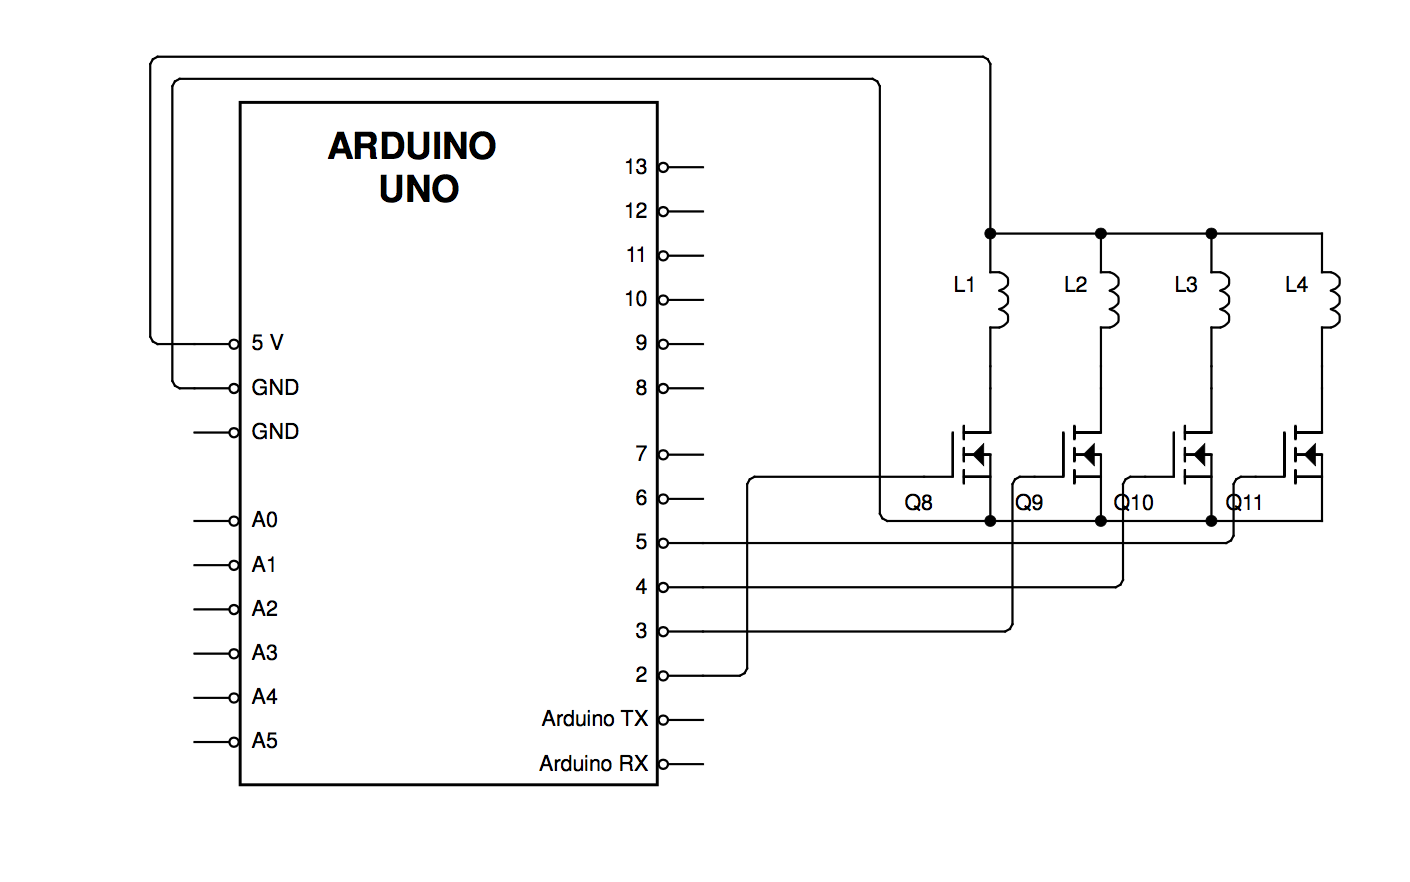
\includegraphics[width=13cm]{figures/CIRCUITS/steppermotorFinal.png}
	\caption{Et billede af kredsløbet for den retningsregulerende kreds.}
	\label{kreds:retning}
\end{figure}
I vores retningsregulerende kreds, har vi valgt at benytte en stepper motor, til at styre hvilken vinkel bolden skydes ud i. Her der bliver der brugt en ekstern strømforsyning på $\SI{5}{V}$, så der kan løbe nok strøm igennem spolerne i stepper motoren. For at bruge den eksterne strømforsyning bruger vi MOSFETs som digitale switches.
\todo{lav kredsen om igen, således at dioden over mosfettet er med, se MOSFET}
\subsection{Komponenter}
\subsubsection{N-Channel power MOSFET - F12N10L}
\begin{figure}[H]
	\centering
    \frame{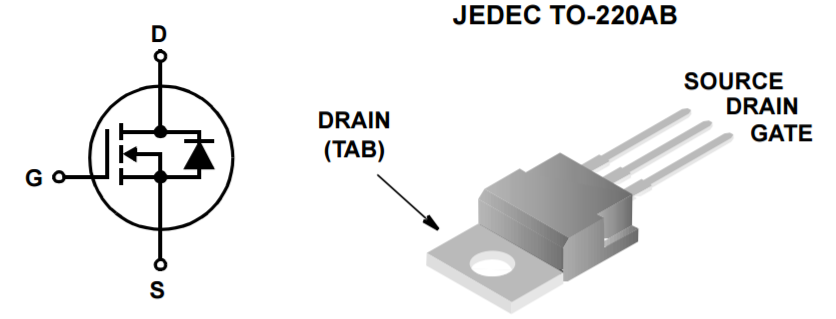
\includegraphics[width=10cm]{figures/komponenter/F12N10L.png}}
	\caption{Pindiagram og symbol af F12N10L. Kilde:\cite{kompMOSFET}}
	\label{fig:kompMOSFET}
\end{figure}
På \Cref{fig:kompMOSFET} er der et symbol og pindiagram over MOSFET komponenten.
Denne MOSFET er bygget til $\SI{5}{V}$ logik, samt har det en lav rise og fall time på et par hundrede nanosekunder og således vil det fungerer fint for en steppermotor. Databladet vi har benyttet kan findes i kilde \cite{kompMOSFET}. 
\todo{skriv om spændingsreguleret - derfor er det godt med arduino}

\subsubsection{Stepper motor - RS191-8328}
\begin{figure}[H]
	\centering
    \frame{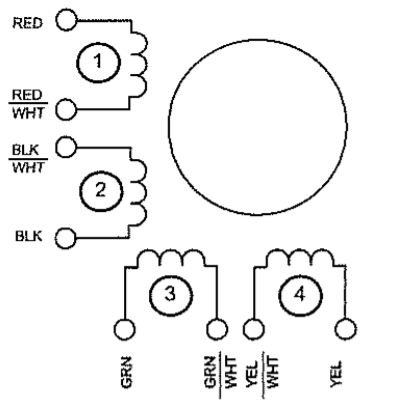
\includegraphics[width=10cm]{figures/komponenter/RS191-8328.png}}
	\caption{Diagram af RS191-8328. Kilde: \cite{kompstepmotor}}
	    \label{fig:kompstepper}
\end{figure}

\todo{Har brug for noget tekst under billedet}

\subsubsection{Arduino}
Se afsnit \ref{sec:arduino}.

\subsection{Teori}
\subsubsection{MOSFET}
Vi benyttede MOSFET for at få en højere strøm igennem spolerne end Arduinoen kan levere. Med en MOSFET kan man kontrollere hvor meget strøm der løber gennem Gate til Source, med spændingsfaldet over Drain og Source. Dette gør en MOSFET optimal som en digital switch. 
\subsubsection{Stepper motor}
Vi benyttede en stepper motor til at styre hvor meget vi drejer kanonen. En stepper motor fungere ved at vi har et vis antal "steps" på en omdrejning. Man kan sende strøm gennem en af spolerne, som så vil trække stepper motoren et "step" frem eller tilbage. Man sender så skiftevis strøm igennem spolerne, for at få stepper motoren til at forsætte i en retning. Vores stepper motor har 200 "steps" på en omdrejning. 
% HVILKET -POLAR ER DET??
\todo{Husk at angive Uni-polar eller Bipolar ***}
%\subsection{Beregninger}

\subsection{Test}
Vi benyttede et Stepper library fra firmaet Arduinos hjemmeside\cite{steppercode:stepbystep}. Koden kan ses på Figur ~\ref{fig:steptest}. \todo{References fungerer meget underligt. Burde sige Figur 10}

% ---------------------BEGIN CODE
\begin{figure}[H] 
\caption{Kode til steppermoter for at angive antal steps der skal roteres}
\label{fig:steptest}
\begin{lstlisting}
#include <Stepper.h>
// Antallet af steps på vores motor
const int stepsPerRevolution = 200;  

// Initialiserer stepper biblioteket i pin 2 til 5:
Stepper myStepper(stepsPerRevolution, 2, 3, 4, 5);

// Antallet af steps motoren har taget
int stepCount = 0;         

void setup() {
//Initialiserer serial porten
  Serial.begin(9600);
}

void loop() {
  // Step et step:
  myStepper.step(1);
  Serial.print("steps:");
  Serial.println(stepCount);
  stepCount++;
  delay(500);
}
\end{lstlisting}
\end{figure}
% -------------------END CODE

Det fungerede fint efter hensigten og vi kunne let styre antallet af steps

% Hastighed 50